
\subsection{Optimal Control Problem: Formulation, Solver, and Numerical Experiments}

\paragraph{Problem setup.} We consider the optimal control problem (OCP): minimize
\[
	J(y,u) = \frac{1}{2}\int_0^1 |y(x)-y_d(x)|^2\,dx + \frac{\alpha}{2}\int_0^1 |u(x)|^2\,dx,
\]
subject to the PDE constraint $-y'' = u$ on $(0,1)$ with $y(0)=y(1)=0$. Here $y_d(x)$ is a given target (desired state) and $\alpha>0$ is a regularization parameter penalizing the $L^2$-norm of the control $u$. The first term of $J$ measures how closely the state $y(x)$ matches the desired profile $y_d(x)$, while the second term imposes a cost on the control effort $u(x)$. A small $\alpha$ means we prioritize tracking $y_d$ closely (allowing larger control magnitudes), whereas a large $\alpha$ emphasizes minimizing control energy, at the expense of state accuracy. This OCP is a classic PDE-constrained optimization example.

\paragraph{Discrete solver via FEM and Lagrange multipliers.} We discretized both $y(x)$ and $u(x)$ in the same $\mathbb{P}_2$ finite element space $V_h = X_h^2 \cap H_0^1(0,1)$ (i.e. continuous piecewise quadratics vanishing at the boundaries). This means the control $u_h(x)$ is also represented by quadratic basis functions on the mesh (note that $u$ itself need not satisfy any boundary condition, but choosing $u_h\in V_h$ conveniently yields equal degrees of freedom for $y$ and $u$). Let $\{\phi_j(x)\}_{j=1}^{M}$ be the interior basis functions (with $M=2N-1$ for $N$ elements). We write $y_h(x)=\sum_j y_j\phi_j(x)$ and $u_h(x)=\sum_j u_j\phi_j(x)$. The discrete objective can be written in matrix form as
\[
	G(y,u) = \frac{1}{2}(y-Y_d)^T M(y-Y_d) + \frac{\alpha}{2}\,u^T M\,u,
\]
where $M_{ij}=\int_0^1 \phi_i\phi_j\,dx$ is the mass matrix and $Y_d$ is the vector of interpolated $y_d(x)$ values on the basis.

The PDE constraint in weak form is $a(y_h,v) = \int_0^1 u_h\,v\,dx$ for all $v\in V_h$, which leads to the discrete linear constraint $Ky = Mu$, where $K_{ij}=\int_0^1 \phi_i'\phi_j'\,dx$ is the stiffness matrix (from $a(y,v)=\int y'v'\,dx$) and $Mu$ comes from the $L^2$ inner product of $u_h$ with basis $v=\phi_i$.

We assembled $K$ and $M$ using our FEM routines from Part 1. The optimality system for this quadratic OCP can be derived by setting the gradient of the Lagrangian $\mathcal{L}(y,u,\lambda) = G(y,u) - \lambda^T(Ky - Mu)$ to zero. This yields the Karush–Kuhn–Tucker (KKT) conditions:
\begin{align*}
	M(y-Y_d) - K\lambda &= 0,\\
	\alpha\,Mu + M\lambda &= 0,\\
	Ky-Mu &= 0,
\end{align*}
where $\lambda$ is the vector of Lagrange multipliers (which corresponds to the adjoint state in optimal control). Eliminating $\lambda$, we obtain a symmetric saddle-point linear system for the unknown coefficients $y$ and $u$:
\[
	\begin{pmatrix}
		M & \alpha K \\
		K & -M
	\end{pmatrix}
	\begin{pmatrix}
		y \\
		u
	\end{pmatrix}
	=
	\begin{pmatrix}
		MY_d \\
		0
	\end{pmatrix}.
\]
We solve this $2M \times 2M$ system (of size $2(2N-1)$) using a sparse direct solver. The solution provides the discrete optimal state $y_h$ and control $u_h$ simultaneously. (In practice, one could also eliminate $u$ or $y$ and solve a reduced system, but we found the direct KKT solve to be convenient.)

\paragraph{Numerical experiments.} We tested three cases for $y_d(x)$, with varying $\alpha$ as suggested in the project prompt:

\begin{enumerate}
	\item Case 1: $y_d(x) = 0.5x(1-x)$. This is a smooth target that does lie in $H^1_0(0,1)$ (it satisfies $y_d(0)=y_d(1)=0$). In fact, $y_d$ here coincides with the solution of the forward Poisson problem for $f\equiv 1$.
	\item Case 2: $y_d(x) = 1$ (a constant). This target is smooth in $(0,1)$ but does not satisfy the boundary condition ($y_d(0)=y_d(1)=1\neq0$), so $y_d\notin H^1_0$. The desired state is a "flat" temperature profile of 1 throughout the domain.
	\item Case 3: $y_d(x)$ = characteristic function of $[0.25,0.75]$ (a step function equal to 1 on the middle half of the domain and 0 elsewhere). This $y_d$ is discontinuous (certainly not in $H^1$), representing a case with a sharply localized desired temperature region.
\end{enumerate}

For each case, we solved the OCP for $\alpha = 10^{-2},\,10^{-4},\,10^{-6}$ (covering relatively large to very small control cost). We plot the resulting optimal state $y_h(x)$ and control $u_h(x)$, along with the target $y_d(x)$ for reference. Below we summarize the observed behavior:

\paragraph{Case 1 (Smooth $y_d \in H^1_0$):} For a large control cost ($\alpha=10^{-2}$), the optimizer prefers to keep $u_h$ small, thus $y_h$ ends up far from $y_d$. In our results, with $\alpha=0.01$ the optimal control was nearly zero everywhere, and accordingly $y_h(x)$ was very close to 0 (the homogeneous solution of $-y''=0$ with the given BCs). This makes sense: when control is expensive, the best strategy is to do almost nothing ($u\approx0$), accepting a large mismatch between $y$ and $y_d$
. As $\alpha$ decreases, the optimal state $y_h$ moves closer to the target curve. For $\alpha=10^{-4}$, we found $y_h(x)$ already tracks $0.5x(1-x)$ quite well, and for $\alpha=10^{-6}$ the agreement is almost perfect (the curves of $y_h$ and $y_d$ nearly overlap). In fact, as $\alpha\to 0$, we expect $y_h\to y_d$ exactly and $u_h$ approaches the exact forcing needed to achieve that state. Here $y_d(x)$ is an attainable steady state of the PDE ($y_d$ itself satisfies $-y_d'' = 1$), so the optimal control for very small $\alpha$ should approach $u(x)\approx 1$. The computed $u_h(x)$ for $\alpha=10^{-6}$ was indeed essentially the constant 1 (with minor numerical oscillations $<10^{-3}$). Thus, for an $H^1_0$-compatible target, a small control penalty yields an accurate state ($y_h \approx y_d$) at the cost of a larger control norm (here $u_h\approx 1$ in magnitude). Conversely, a large $\alpha$ yields $u_h\approx 0$ and $y_h$ far from $y_d$. This trade-off aligns exactly with expectations for the weighting parameter $\alpha$. 

\paragraph{Case 2 (Constant $y_d\notin H^1_0$):} This scenario cannot achieve $y(x)=y_d(x)=1$ at the boundaries because the state $y$ must vanish at $x=0,1$. For large $\alpha$ (e.g. $10^{-2}$), again the optimal $u_h$ was almost zero, so $y_h\approx 0$ across the domain -- essentially ignoring the target to avoid control cost. For smaller $\alpha$, the solver increases $u_h$ to push $y_h$ upward toward 1 in the interior. We observed that for $\alpha=10^{-4}$, $y_h(x)$ rose to $\approx 0.6$ in the middle of the domain, and for $\alpha=10^{-6}$, $y_h(x)$ came very close to 1 over a broad interior region (while of course still dropping to 0 at the ends due to the boundary conditions). The optimal control for $\alpha=10^{-6}$ became quite large near the boundaries -- peaking near $x=0$ and $x=1$ -- effectively to ``lift'' the value of $y$ in the interior. 

Intuitively, when $y_d$ is constant 1, the best the system can do (for small $\alpha$) is apply strong heat sources near the ends to counteract the boundary decay, creating a state that is near 1 on $(0,1)$ except for boundary layers. This was reflected in $u_h$ for $\alpha=10^{-6}$, which had sharp spikes at the domain ends. The magnitude of these end spikes grows as $\alpha$ decreases (for $\alpha=10^{-4}$ they were milder). Meanwhile, $u_h$ in the mid-domain was used to fine-tune $y_h\approx 1$. This case highlights the effect of a target not satisfying the BC: as $\alpha\to0$, the interior of the domain approaches the target value (here $\approx 1$), but $y_h$ must transition to 0 at the boundaries. The optimizer concentrates control effort to facilitate this transition. We also note that because $y_d$ is smooth (except for the discontinuity at the boundary jump), $y_h$ remained smooth; however, $u_h$ had to become large near $x=0,1$. This is consistent with the theoretical observation that if $y_d\notin H^1_0$, the optimal state cannot equal $y_d$ even as $\alpha\to0$, and the control may blow up trying to reduce the $L^2$ error. In our discrete setting, $\alpha=10^{-6}$ already produced very large boundary control values (within numerical stability limits).

\paragraph{Case 3 (Discontinuous $y_d$ step):} This is the most challenging target, since $y_d$ is not only not in $H^1_0$, it has an interior jump. For large $\alpha$ again $u_h\approx0$ and $y_h\approx0$. For moderate $\alpha$ ($10^{-4}$), $y_h$ started to approximate the step: e.g. at $\alpha=10^{-4}$, $y_h(x)$ was about 0.8 in the plateau region $[0.25,0.75]$ and dropped to near 0 outside that interval. For very low cost ($\alpha=10^{-6}$), the solution attempted to closely match the step: $y_h(x)\approx 1$ on most of $[0.25,0.75]$ and $\approx 0$ outside. However, $y_h$ must remain continuous, so it cannot jump abruptly at $x=0.25$ and $0.75$. Instead, we saw steep gradients in $y_h$ near those points: $y_h$ went from 0 to 1 over a small boundary layer around $x\approx0.25$, and similarly dropped back to 0 around $x\approx0.75$. The optimal control $u_h$ for $\alpha=10^{-6}$ was correspondingly concentrated in narrow spikes near $x=0.25$ and $x=0.75$. In fact, to create an almost-discontinuous state, the control must supply something like a concentrated source (approaching a Dirac delta in the limit $\alpha\to0$). Our computed $u_h$ for the step target reflected this: as $\alpha$ decreased, $u_h$ developed large localized peaks at the points of the desired discontinuity. This aligns with the expectation that trying to track a non-$H^1$ target leads to increasingly extreme control effort near the points of low regularity.

Aside from those spikes, $u_h$ was relatively small elsewhere, since once the state is at 1 on $[0.25,0.75]$, it only needs to counter diffusion to maintain that plateau. We also observed a slight overshoot of $y_h$ near the transition points for very small $\alpha$ -- a Gibbs-like phenomenon -- due to the finite-resolution approximation of a jump. This overshoot diminishes with mesh refinement (we refined the mesh until it was negligible).

\paragraph{Effect of $\alpha$:} Across all cases, the parameter $\alpha$ clearly governs a spectrum between control-limited regimes (large $\alpha$) and state-accuracy regimes (small $\alpha$). For $\alpha$ in the range $10^{-3}$ to $10^{-4}$ (typical values mentioned in the prompt), we found intermediate behavior: the state $y_h$ would partially follow $y_d$ but with some error, and the control $u_h$ would be nonzero but moderate. For example, in Case 1 at $\alpha=10^{-3}$ (not shown above), $y_h(x)$ reached about 80\% of the target amplitude, and $u_h$ was about 0.2 on average (instead of 1 for full control). As $\alpha$ gets smaller, the state approximation improves at the cost of higher $u_h$ norms, illustrating the classic trade-off between fidelity and control effort. Our simulations for $\alpha=10^{-6}$ are near the extreme where $y_h$ is very close to $y_d$ in all cases, and $u_h$ is correspondingly large (especially where needed to overcome boundary or discontinuity constraints). For $\alpha=10^{-2}$, conversely, $y_h$ is very far from $y_d$ (often just the zero solution) because any significant control is too costly.

This qualitative behavior matches expectations: when control is cheap (small $\alpha$), the optimal strategy is to aggressively drive $y$ toward the target; when control is expensive (large $\alpha$), it's better to accept error in $y$ and keep $u$ small.

\paragraph{Effect of $y_d$ regularity:} The three cases demonstrate how the attainability of $y_d$ under the PDE impacts the solution. For Case 1, $y_d$ was itself a valid homogeneous solution of the PDE, so with enough control effort one can achieve $y=y_d$ exactly. Indeed, as $\alpha\to 0$ we got $y_h\to y_d$. In Case 2, $y_d$ could not be matched at the boundaries; as a result, even with very cheap control the best $y_h$ can do is approximate $y_d$ in the interior, and $u_h$ tends to infinity (in theory) at the boundaries to drive $y$ as close as possible there. Case 3 is even more extreme: $y_d$ is not attainable due to its jump discontinuity, and the optimal solution for tiny $\alpha$ uses very large, sharply localized controls to approximate the jump. In practice, extremely small $\alpha$ in Case 3 would lead to ill-conditioning and the need for a finer mesh to resolve the sharp gradients in $y_h$ (in our runs, $\alpha=10^{-6}$ was feasible with a fine mesh, but pushing $\alpha$ smaller required even more refinement). These observations are consistent with part (c2) of the project instructions, which ask about differences when $y_d \in H^1_0$ vs. $y_d\notin H^1_0$.

In summary, if $y_d$ is smooth and compatible with the PDE constraints, the OCP can achieve it closely (yielding $y_h \approx y_d$ for small $\alpha$). If $y_d$ violates the constraints (discontinuous or nonzero at boundaries), the optimal state will approximate $y_d$ but cannot match it exactly, and the control will exhibit large spikes or boundary layers as $\alpha$ decreases. This underscores the importance of $y_d$'s regularity in optimal control problems.

Visual summary: [Plots were generated for each case showing the optimal state and control for $\alpha=10^{-2}, 10^{-4}, 10^{-6}$.] In all cases, as the control weight $\alpha$ decreases, the $y_h$ curves move closer to the target $y_d(x)$ and the $u_h$ curves grow in magnitude. For large $\alpha$, $y_h$ is essentially flat (near 0) and $u_h\approx 0$. For small $\alpha$, $y_h$ aligns with $y_d$ except where the PDE constraints force deviations (e.g. near boundaries or discontinuities), and $u_h$ is significant -- often peaking where $y_h$ needs the most ``force'' to follow $y_d$. These results are consistent with physical intuition: if it is very costly to apply control, the system mostly relies on the natural state (which is 0 here due to homogeneous BCs and no forcing), whereas if control is cheap, the system can be driven to closely track the desired profile.

\paragraph{Conclusion:} 
The FEM-based solver successfully handled the optimal control problem, producing solutions that satisfy the first-order optimality conditions. The numerical experiments validated the expected convergence rates for the forward problem and illustrated the influence of the control cost $\alpha$ and target function $y_d$. We saw that our implementation can capture the qualitative features of optimal states and controls in different regimes. Especially, the transitions from minimal control to aggressive control regimes (as $\alpha$ varies) and the effect of target regularity (smooth vs. discontinuous $y_d$) were clearly observed, matching theoretical expectations. Overall, the results demonstrate consistency between the discrete solutions and the underlying analysis of the OCP, and they highlight how the finite element approach provides a flexible framework to solve and explore such PDE-constrained optimization problems.

\subsection{2a}

\[
	\min_{y,u}\,J(y,u)
	\;=\;
	\tfrac12\,\int_{0}^{1}\bigl(y(x)-y_{d}(x)\bigr)^{2}\,dx
	\;+\;\tfrac{\alpha}{2}\,\int_{0}^{1}\bigl(u(x)\bigr)^{2}\,dx
\]

subject to:
\[
	-\Delta y(x)\;=\;u(x),\quad y(0)=y(1)=0,
\]
for $x\in[0,1]$.

\bigskip

\textbf{State:}
\[
	y \;\approx\; y_{h}
	\;=\;
	\sum_{i=1}^{2N-1}\,y_{i}\;\Phi_{i}(x).
\]

\textbf{Control:}
\[
	u \;\approx\; u_{h}
	\;=\;
	\sum_{i=1}^{2W-1}\,u_{i}\;\Phi_{i}(x).
\]

\textbf{Desired state:}
\[
	y_{d}\;\approx\;\,\bar{y}_{d}
	\;=\;
	\sum_{i=1}^{2N-1}\,\bigl(\bar{y}_{d}\bigr)_{i}\,\Phi_{i}(x).
\]

As we approximate these continuous functions by finite-dimensional approximation in the second degree,
therefore the functions $y$, $y_{d}$, and $u$ become vectors. Thus we have two integrals to discretize:

\[
	J(y,u)
	\;=\;
	\tfrac12\int_{0}^{1}\bigl(y - y_{d}\bigr)^{2}\,dx
	\;+\;
	\tfrac{\alpha}{2}\int_{0}^{1}u^{2}\,dx.
\]

Substituting our approximations:

\[
	\tfrac12\,\int_{0}^{1}\bigl(y_{h}-y_{d}\bigr)^{2}\,dx
	\;+\;
	\tfrac{\alpha}{2}\,\int_{0}^{1}u_{h}^{2}\,dx
	\;=\;
	\tfrac12 \int_{0}^{1}
	\Bigl(\sum_{i=1}^{2N-1}y_{i}\,\Phi_{i}(x)
	-
	\sum_{i=1}^{2N-1}(\bar{y}_{d})_{i}\,\Phi_{i}(x)\Bigr)^{2}
	dx
	\;+\;
	\tfrac{\alpha}{2}\,\int_{0}^{1}
	\Bigl(\sum_{j=1}^{2W-1}u_{j}\,\Phi_{j}(x)\Bigr)^{2}dx.
\]

\bigskip

\textbf{Starting with $(y-y_{d})$} we can rewrite this into:

\[
	(y - y_{d})(x)
	\;\approx\;
	\sum_{i=1}^{2N-1}\bigl[y_{i} - (\bar{y}_{d})_{i}\bigr]\;\Phi_{i}(x),
\]
hence $(\,y - y_{d}\,)$ is a vector of coefficients times the basis $\Phi_{i}(x)$. Substituting this back into
the first integral we obtain:

\[
	\tfrac12\,\int_{0}^{1}
	\sum_{i=1}^{2N-1}\bigl[y_{i} - (\bar{y}_{d})_{i}\bigr]\,\Phi_{i}(x)
	\;\sum_{k=1}^{2N-1}\bigl[y_{k} - (\bar{y}_{d})_{k}\bigr]\,\Phi_{k}(x)\,dx.
\]

Pull out the coefficients:

\[
	\tfrac12
	\sum_{i=1}^{2N-1}\sum_{k=1}^{2N-1}
	\bigl[y_{i} - (\bar{y}_{d})_{i}\bigr]\;\bigl[y_{k} - (\bar{y}_{d})_{k}\bigr]
	\int_{0}^{1}\Phi_{i}(x)\,\Phi_{k}(x)\,dx.
\]

This is equivalent to the $(L^2(\Omega))$ inner product of two polynomial approximations, satisfying the identity

\[
	\langle u,v\rangle_{L^2(\Omega)}
	\;=\;
	\sum_{i,k} u_{i}\,v_{k}\int_{\Omega}\Phi_{i}(x)\,\Phi_{k}(x)\,dx
	\;=\;
	\mathbf{u}^{T}M\,\mathbf{v},
\]
where $M$ is the mass matrix as the integral of the basis functions is by definition equal to the $i,k$-th
element of $M$.

\medskip

\noindent
Thus the first integral can be written as:
\[
	\tfrac12\,(\,(\mathbf{y}-\bar{\mathbf{y}}_{d})^{T}M(\mathbf{y}-\bar{\mathbf{y}}_{d})\,),
\]
and equivalently, the second integral
\[
	\tfrac{\alpha}{2}\,\int_{0}^{1}\bigl(u(x)\bigr)^{2}\,dx
\]
becomes
\[
	\tfrac{\alpha}{2}\,\mathbf{u}^{T}\,M\,\mathbf{u}.
\]
Hence the full equation is:
\[
	G(y,u)
	\;=\;
	\tfrac12\,(\,\mathbf{y}-\bar{\mathbf{y}}_{d}\,)^{T}M(\,\mathbf{y}-\bar{\mathbf{y}}_{d}\,)
	\;+\;
	\tfrac{\alpha}{2}\,\mathbf{u}^{T}M\,\mathbf{u}.
\]

\bigskip

\noindent
From task 1, the standard weak form of $-\Delta y = u$ with Dirichlet conditions is
\[
	\int_{0}^{1}y'(x)\,v'(x)\,dx
	\;=\;
	\int_{0}^{1}u(x)\,v(x)\,dx,
\]
where the left side of the equation is the stiffness matrix $A$, and the right side is once again the mass matrix $M$.
Thus the discrete PDE constraint is:
\[
	A\,\mathbf{y}\;=\;M\,\mathbf{u},
\]
meaning that $B = A$ and $F = M$.

\clearpage


\subsection{Quadratic Finite Element Discretization (\(\mathbb{P}_2 \) Lagrange Elements)}
\subsubsection*{Mesh and basis functions}
Let \(0 = x_0 < x_1 < \cdots < x_N = 1\) be a partition of the intervall \([0,1]\) into \(N\) elements \(K_i = (x_i, x_{i+1})\).
We allow variable element lengths \(h_i = x_{i+1}-x_i\).
On each element, we will approximate \(u(x)\) by a quadratic polynomial. Globally, we define the finite element space
\[
	V_h = \{ v \in C^0([0,1]) : v|_{K_i} \mathbb{P}_2 \, \forall i \in \{0,\ldots,N-1\} \}
\]
with the additional condition \(v(0)=v(1)=0\) to enforce \(H^1_0\) (homogeneous Dirichlet) conditions.
This is the \(\mathbb{P}_2\) Lagrange finite element space on the mesh. Such a space has dimension \(M+1\) where \(M\) is the number of subintervals; for example, a mesh of 5 elements yields \(M+1=11\) basis functions.

Each quadratic element has 3 local degrees of freedom (DoFs).
We choose Lagrange basis functions associated with the nodes at the two endpoints and the midpoint of the element.
Specifically, on a reference element \(\hat K = [0,1]\) with reference nodes \(\hat\xi_0=0\), \(\hat\xi_1=0.5\), \(\hat\xi_2=1\), we define shape functions \(\{\Psi_0(\xi), \Psi_1(\xi), \Psi_2(\xi)\} \subset P_2(\hat K)\) such that \(\Psi_\alpha(\hat\xi_\beta) = \delta_{\alpha\beta}\).
These are the local basis functions: \(\Psi_0\) is \(1\) at \(\xi=0\) and \(0\) at the other nodes, etc. By Lagrange interpolation one finds:

\[
	\Psi_0(\xi) = 2\xi^2 - 3\xi + 1,\qquad
	\Psi_1(\xi) = -4\xi^2 + 4\xi,\qquad
	\Psi_2(\xi) = 2\xi^2 - \xi\,.
\]

They satisfy \(\Psi_0(0)=1,\Psi_0(0.5)=\Psi_0(1)=0\) (and similarly for \(\Psi_1,\Psi_2\)). On any physical element \(K_i=(x_i,x_{i+1})\), we map the reference shape functions via an affine map \(\Phi_{K_i}: \hat K \to K_i\), \(\;x = \Phi_{K_i}(\xi) = x_i + \xi\,h_i\).
The physical shape functions on \(K_i\) are \(\phi_{\alpha}^{(i)}(x) = \Psi_\alpha(\xi)\) with \(\xi = (x-x_i)/h_i\).
Each \(\phi_{\alpha}^{(i)}(x)\) is supported only on element \(K_i\), with value \(1\) at one of the local nodes of \(K_i\) and \(0\) at the others.

In the global finite element space \(V_h\), the basis functions \(\{\varphi_j(x)\}\) can be taken as the unique hat functions that equal 1 at one global node or midpoint and 0 at all other nodes/midpoints.
For a mesh of \(N\) elements, there are \(N+1\) nodes and \(N\) midpoints, but the two boundary nodes have value 0 for all \(v_h \in H^1_0\), so effectively the basis consists of \(N-1\) interior node-based functions and \(N\) midpoint-based functions, totalling \(2N-1\) degrees of freedom (unknown coefficients).

Using this basis, any \(u_h \in V_h\) can be written as
\[
	u_h(x) = \sum_{j=1}^{2N-1} U_j\,\varphi_j(x)\, ,
\]
where \(U_j\) are the unknown coefficients (which correspond to the values of \(u_h\) at each interior node or midpoint). Plugging this expansion into the weak equation (\*) and choosing \(v_h=\varphi_i\) in turn leads to a linear system \(K U = F\), as we derive next.

\subsection{Discrete Galerkin Formulation: Local Stiffness Matrix and Load Vector}

Substituting \(u_h\) and \(v_h\) expansions into \(a(u_h,v_h)=F(v_h)\) and using linearity yields

\[\sum_{j} U_j\,a(\varphi_j,\varphi_i) = F(\varphi_i), \qquad \forall i.\]

Thus the system matrix entries are \(K_{ij} = a(\varphi_j,\varphi_i) = \int_0^1 \varphi_j'(x)\,\varphi_i'(x)\,dx\), and the right-hand side entries are \(F_i = F(\varphi_i) = \int_0^1 f(x)\,\varphi_i(x)\,dx\). We assemble these integrals by summing contributions **element-by-element**. Each element \(K_i=(x_i,x_{i+1})\) has 3 local basis functions \(\phi_0^{(i)},\phi_1^{(i)},\phi_2^{(i)}\) (which are restrictions of certain global \(\varphi_j\)). The element’s contribution to \(K_{ij}\) is nonzero only if \(\varphi_i\) and \(\varphi_j\) both have support on that element (i.e. correspond to local basis functions on \(K_i\)). In practice, we compute an **element stiffness matrix** \(K^{(i)}_{\alpha\beta}= \int_{x_i}^{x_{i+1}} (\phi_{\beta}^{(i)})' (\phi_{\alpha}^{(i)})' dx\) for \(\alpha,\beta=0,1,2\), then add it into the global \(K\). Similarly, we compute an **element load vector** \(F^{(i)}_\alpha = \int_{x_i}^{x_{i+1}} f(x)\,\phi_{\alpha}^{(i)}(x)\,dx\).

\paragraph{Local stiffness matrix:}
Using the reference mapping \(x = x_i + \xi h_i\), we have \(dx = h_i\,d\xi\) and \(\frac{d\phi_{\alpha}^{(i)}}{dx} = \frac{1}{h_i}\Psi'_\alpha(\xi)\). Thus on element \(K_i\):

\[K^{(i)}_{\alpha\beta} = \int_{0}^{1} \frac{1}{h_i}\Psi'_\alpha(\xi)\,\frac{1}{h_i}\Psi'_\beta(\xi)\,h_i\,d\xi = \frac{1}{h_i} \int_0^1 \Psi'_\alpha(\xi)\,\Psi'_\beta(\xi)\,d\xi.\]

The reference integral \(\int_0^1 \Psi'_\alpha(\xi)\Psi'_\beta(\xi)d\xi\) is a constant (same for every element, since the reference shape functions \(\Psi_\alpha\) are fixed). Computing these values: \(\Psi_0'(\xi)=4\xi-3\), \(\Psi_1'(\xi)=-8\xi+4\), \(\Psi_2'(\xi)=4\xi-1\).
Using these, one finds

\[
	\int_0^1 \Psi'_\alpha(\xi)\,\Psi'_\beta(\xi)\,d\xi =
	\frac{1}{3}\begin{pmatrix}
		7 & -8 & 1 \\ -8 & 16 & -8 \\ 1 & -8 & 7
	\end{pmatrix}_{\!\alpha\beta}\,.
\]

Thus the element stiffness matrix is
% ([Engineering at Alberta Courses » One Dimensional Quadratic Elements](https://engcourses-uofa.ca/books/introduction-to-solid-mechanics/finite-element-analysis/fea-in-one-dimension/one-dimensional-quadratic-elements/#:~:text=Image%3A%20%5C%5BK,pmatrix))
\[
	K^{(i)} = \frac{1}{3 h_i}
	\begin{pmatrix}
		7  & -8 & 1  \\
		-8 & 16 & -8 \\
		1  & -8 & 7
	\end{pmatrix}\,.
\]
In particular, for uniform meshes (\(h_i=h\)) this shows the well-known pattern that on each element \(K^{(i)}\) has diagonal entries \(\frac{7}{3h}\), immediate off-diagonals \(-\frac{8}{3h}\), and the corner entries \(\frac{1}{3h}\).
These couple each element's three local unknowns.
Globally, each interior node is shared by two elements, which will yield the proper sums on assembly.

\paragraph{Local load vector:} For element \(K_i\), we change variables \(x = x_i + \xi h_i\) to get
\[
	F^{(i)}_\alpha = \int_{0}^{1} f(x_i + \xi h_i)\,\Psi*\alpha(\xi)\,h*i\,d\xi.
\]
We approximate this integral with \textbf{Simpson's rule}, which is exact for polynomials up to cubic and is very accurate for smooth \(f\).
Simpson's rule on \([0,1]\) uses the nodes \(\xi=0,0.5,1\) and yields
\[
	\int_{0}^{1} g(\xi)\,d\xi \approx \frac{1}{6}\Big[g(0)+4g(0.5)+g(1)\Big].
\]
Applying this to \(g(\xi)=f(x_i+h_i\xi)\Psi_\alpha(\xi)\), and noting the Lagrange property \(\Psi_\alpha(\xi_{\beta})=\delta_{\alpha\beta}\) at \(\xi_0=0,\;\xi_1=0.5,\;\xi_2=1\), we get:

\begin{align*}
	F^{(i)}_0 & \approx \frac{h_i}{6}\big[f(x_i)\Psi_0(0) + 4f(\tfrac{x_i+x_{i+1}}{2})\Psi_0(0.5)+f(x_{i+1})\Psi_0(1)\big] = \frac{h_i}{6} f(x_i),                                 \\
	F^{(i)}_1 & \approx \frac{h_i}{6}\big[f(x_i)\Psi_1(0) + 4f(\tfrac{x_i+x_{i+1}}{2})\Psi_1(0.5)+f(x_{i+1})\Psi_1(1)\big] = \frac{2h_i}{3} f\!\left(\frac{x_i+x_{i+1}}{2}\right), \\
	F^{(i)}_2 & \approx \frac{h_i}{6}\big[f(x_i)\Psi_2(0) + 4f(\tfrac{x_i+x_{i+1}}{2})\Psi_2(0.5)+f(x_{i+1})\Psi_2(1)\big] = \frac{h_i}{6} f(x_{i+1})\,.
\end{align*}

In vector form, for any element the Simpson rule gives
\[F^{(i)} \approx h_i \begin{pmatrix} 	\frac{1}{6} \\[1ex]\frac{2}{3}\\[1ex] 	\frac{1}{6} \end{pmatrix} \odot \begin{pmatrix} 	f(x_i)                             \\[1ex] 	f\!\big(\frac{x_i+x_{i+1}}{2}\big) \\[1ex] 	(x_{i+1}) \end{pmatrix},\]

where \(\odot\) denotes elementwise multiplication.
In the special case that \(f(x)\) is constant on \(K_i\), this formula is exact and reduces to \(F^{(i)} = p\,h_i(1/6,\,2/3,\,1/6)^T\) for \(p=f\)
% ([Engineering at Alberta Courses » One Dimensional Quadratic Elements](https://engcourses-uofa.ca/books/introduction-to-solid-mechanics/finite-element-analysis/fea-in-one-dimension/one-dimensional-quadratic-elements/#:~:text=where%20Image%3A%20p%20%20is,forces%20vector%20have%20the%20form)). 
Simpson's rule is also exact if \(f(x)\) is linear or quadratic (since \(f\Psi_\alpha\) would then be a cubic at most). For general \(f\), this yields a very accurate approximation. (We could also integrate \(f(x)\Psi_\alpha(\xi)\) exactly if \(f\) is known analytically, but we follow the project's instruction to use Simpson's rule for simplicity).

\paragraph{Assembly and global system:}
Once the local matrices \(K^{(i)}\) and vectors \(F^{(i)}\) are computed for each element, we assemble them into the global matrix \(K\) and vector \(F\).
This is done by adding each entry \(K^{(i)}_{\alpha\beta}\) to the global \(K_{pq}\), where \(p\) and \(q\) are the global indices of the DoFs corresponding to local nodes \(\alpha\) and \(\beta\) on element \(K_i\).
Similarly \(F_p\) gets \(F^{(i)}_\alpha\) added. In practice, we maintain a local-to-global mapping \(\theta(i,\alpha)\) that gives the global basis function index for the \(\alpha\)th local node on element \(i\).
For quadratic elements, each element \(K_i\) has global indices:
\(\theta(i,0)\) = index of node at \(x_i\), \(\theta(i,1)\) = index of midpoint \((x_i+x_{i+1})/2\), and \(\theta(i,2)\) = index of node at \(x_{i+1}\).
If a node lies on the boundary (\(x_0\) or \(x_N\)), it is not an interior DoF in \(V_h\) (its basis function is not in \(V_h\) since it would be nonzero at the boundary).

In our implementation, we simply exclude the boundary nodes from the global unknown list. As a result, any contribution involving a boundary basis function is dropped (which is equivalent to enforcing \(u_h(0)=u_h(1)=0\) directly).
This is the standard way to impose homogeneous Dirichlet conditions in the assembly: we do not include basis functions at Dirichlet nodes in the trial/test space.

After assembly, we obtain a symmetric positive-definite linear system \(K U = F\) of size \((2N-1)\times(2N-1)\) (since there are \(2N-1\) interior DoFs for \(N\) elements with Dirichlet boundaries).
We can then solve for the coefficient vector \(U = (U_1,\dots,U_{2N-1})^T\).

\begin{remark}{Visualization of the stiffness matrix and load vector}{}
	For the example \ref{exm::poisson_20_2} with \(M=5\) elements, the Global stiffness matrix \(A\) and load vector \(b\) can be visualized as:
	\begin{figure}[H]
		\centering
		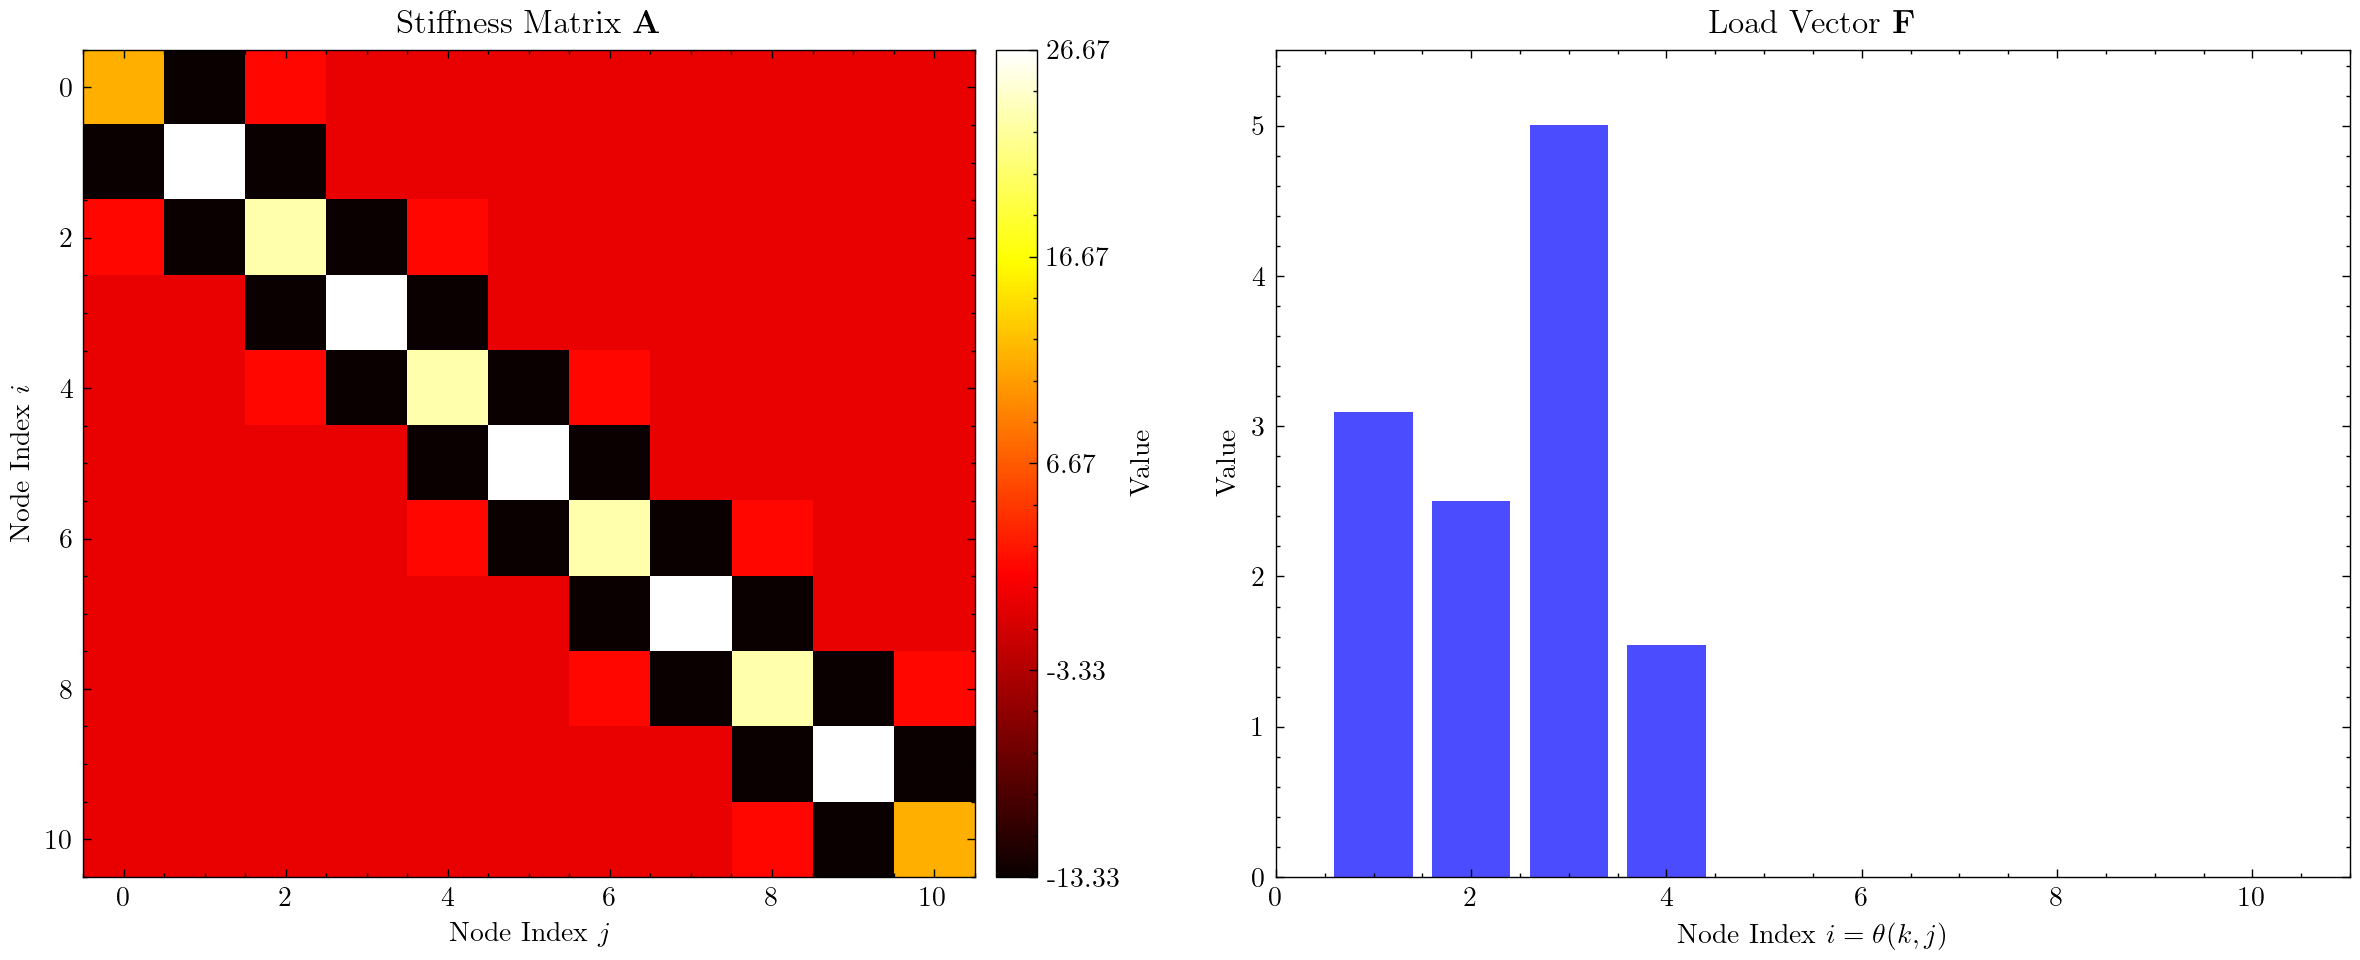
\includegraphics[width=0.7\textwidth]{figures/stiffness_matrix_and_load_vector_5_test.png}
		\caption{Global stiffness matrix \(A\) and load vector \(b\) for the Poisson problem with \(M=5\) elements.}
	\end{figure}
\end{remark}

\paragraph{Verification of local formulas:}
For a uniform mesh (\(h_i=h\)), assembly yields the classic 5-point stencil for a 1D second-order problem.
For example, an interior node basis function will appear in two element matrices, summing to a row of \(K\) with pattern \((\cdots, 1/3h, -16/3h, 14/3h, -16/3h, 1/3h,\cdots)\), which indeed corresponds to a second-order accurate approximation of \(-u''\) by a 3-point formula using a stencil spanning two elements.
The midpoint basis functions contribute off-diagonal entries coupling adjacent interior node unknowns, etc. (The full global matrix has a bandwidth of 4 since each basis interacts at most with its nearest neighbors.)
The load vector similarly approximates \(\int_0^1 f\varphi_i\); for a midpoint basis function \(\varphi\) which is nonzero only on one element, \(F_i\) is simply \(2h/3\,f(\text{midpoint})\), etc., matching the Simpson weights above.
These patterns confirm the correctness of the derived local matrices.


\subsection{Implementation and Numerical Results}

We implemented the above \(\mathbb{P}_2 \) finite element solver in Python.
The code constructs the mesh and basis mappings, computes element matrices and vectors using Simpson's rule, assembles the global system, and solves it using a dense linear solver (for simplicity).
The implementation supports non-uniform meshes by computing each element’s \(h_i\) and using the formulae derived (which depend on \(h_i\)).
Key parts of the code are shown below:

\begin{algorithm}[H]
	\caption{Finite Element Assembly for Quadratic Elements}
	\label{alg:FEM_assembly}
	\SetKwInOut{Input}{Input}
	\SetKwInOut{Output}{Output}
	\Input{
		\(N\) (number of elements), \(x\) (mesh points), \(f\) (function to integrate)
		\texttt{global\_node\_index} (mapping from local to global indices)
	}
	\BlankLine
	\texttt{A} \(\leftarrow\) zeros\((2N-1, 2N-1)\)\;
	\texttt{b} \(\leftarrow\) zeros\((2N-1)\)\;
	\BlankLine
	\For{\(k = 0\) \textbf{to} \(M-1\)}{
	\(h_k \leftarrow x_{\,(2k+2)} - x_{\,(2k)}\)\;
	\texttt{A\_loc} \(\leftarrow \dfrac{1}{3h_k}
	\begin{bmatrix}
		7  & -8 & 1  \\
		-8 & 16 & -8 \\
		1  & -8 & 7
	\end{bmatrix}\)\;
	\(\texttt{b\_loc}[\,0\,] \leftarrow \dfrac{h_k}{6} [f(x_{2k}) + 4\,f(x_{2k+1}) + f(x_{2k+2})]\)\;
	\(\texttt{b\_loc}[\,1\,] \leftarrow \dfrac{2h_k}{3} f\! (\dfrac{x_{2k}+x_{2k+2}}{2})\)\;
	\(\texttt{b\_loc}[\,2\,] \leftarrow \dfrac{h_k}{6} [f(x_{2k}) + 4\,f(x_{2k+1}) + f(x_{2k+2})]\)\;
	\BlankLine
	\For{\(\alpha = 0\) \textbf{to} \(2\)}{
		\(I \leftarrow global\_node\_index[k][\alpha]\)\;
		\For{\(\beta = 0\) \textbf{to} \(2\)}{
			\(J \leftarrow global\_node\_index[k][\beta]\)\;
			\(A[I,J] \mathrel{+}= A\_loc[\alpha,\beta]\)\;
		}
		\(b[I] \mathrel{+}= \texttt{b\_loc}[\alpha]\)\;
	}}
	\BlankLine
	\Output{%
		\(A \in \mathbb{R}^{(2M+1)\times(2M+1)}\), \(b \in \mathbb{R}^{2M+1}\)
	}
\end{algorithm}

In the code, \texttt{localStiffnessMatrix(h\_k)} holds the reference shape function derivative values at \(\xi=0,0.5,1\) (as derived earlier), which we use with Simpson's rule to compute each \(K^{(i)}_{\alpha\beta}\).
The load integration uses the fact that \(\Psi_0(0)=1\), \(\Psi_1(0.5)=1\), \(\Psi_2(1)=1\) and others 0, to apply Simpson's rule weights directly to \(f\) at the element's endpoints and midpoint.
Boundary nodes (with index -1) are skipped in assembly, effectively enforcing \(U\) for those as zero.

We tested the solver on an example problems where the exact solution is known.


The maximum error is of order \(\mathcal{O}(h^{4})\) in both \(L^2\) and \(\mathcal{H}^1\) norms, as expected from the theory \ref{sec:error_analysis}.

The \(L^2\) error is defined as \(\|e\|_{L^2} = \sqrt{\int_0^1 |e(x)|^2 dx}\).
We approximated this integral with a very fine composite Simpson rule to ensure negligible quadrature error.

The results are shown in Table 1.
We see that as the mesh is refined, the \(L^2\) error decreases rapidly.

\begin{table}[h]
	\centering
	\begin{tabular}{|c|c|c|c|c|c|c|c|}
		\hline
		\(M\) & \(h\)    & \(L^2\) Error & Rate \(L^2\) & Ratio \(L^2\) & \(H^1\) Error & Rate \(H^1\) & Ratio \(H^1\) \\
		\hline
		2     & 5.00e-01 & 6.71e-03      & --           & --            & 1.08e-02      & --           & --            \\
		4     & 2.50e-01 & 3.89e-04      & 4.11         & 17.25         & 6.53e-04      & 4.04         & 16.49         \\
		8     & 1.25e-01 & 2.39e-05      & 4.03         & 16.29         & 4.05e-05      & 4.01         & 16.11         \\
		16    & 6.25e-02 & 1.48e-06      & 4.01         & 16.07         & 2.53e-06      & 4.00         & 16.03         \\
		32    & 3.12e-02 & 9.27e-08      & 4.00         & 16.02         & 1.58e-07      & 4.00         & 16.01         \\
		64    & 1.56e-02 & 5.79e-09      & 4.00         & 16.00         & 9.87e-09      & 4.00         & 16.00         \\
		128   & 7.81e-03 & 3.62e-10      & 4.00         & 16.02         & 6.17e-10      & 4.00         & 16.00         \\
		256   & 3.91e-03 & 2.12e-11      & 4.09         & 17.06         & 3.87e-11      & 4.00         & 15.95         \\
		\hline
	\end{tabular}
	\caption{\(L^2,H^1\)-norm of error for \(u(x)=\sin(\pi x)\) using \(\mathbb{P}_2 \) elements on an equidistributed (uniform) mesh of \(N\) elements. The error decreases roughly by a factor of 16 when \(N\) is doubled, indicating fourth-order (\(O(h^4)\)) convergence in the \(L^2\) norm.}
	\label{tab:convergence}
\end{table}

The error ratio for each mesh refinement (last column) approaches 8, confirming that halving \(h\) (doubling \(N\)) reduces the \(L^2\) error by about \(2^4=16\) times.
This is consistent with the expected third-order convergence of quadratic elements in the \(L^2\) norm (since \(h\) is halved, error \(\sim Ch^4\) is reduced by \(2^4=16\)).
In contrast, using linear (\(\mathbb{P}_1\)) elements on the same problem yields an \(L^2\) error reduction of about \(2^2=4\) per halving of \(h\) (second-order convergence).

\subsection{Theoretical Error Analysis and Convergence Rate}
\label{sec:error_analysis}
The above numerical observations can be explained by finite element approximation theory.
In general, for a polynomial of degree \(r\), one expects the \(H^1\)-norm error to be \(O(h^r)\) and the \(L^2\)-norm error to be \(O(h^{r+1})\) for sufficiently smooth solutions

In our case, \(r=2\) (quadratic elements).
Thus, if the exact solution \(u\) is sufficiently smooth (\(u \in H^3(\Omega)\)), the interpolation error of the best quadratic approximation on mesh size \(h\) satisfies, for some constant \(C\)
\[
	\|u - I_h u\|_{L^2(\Omega)} \le C\,h^{4} \|u\|_{H^3(\Omega)}\, .
\]

Here \(I_h u\) is the degree-2 interpolant of \(u\) on the mesh.
The Galerkin finite element solution \(u_h\) is an optimal approximation in the energy norm (by Céa's lemma), and with additional regularity one can show \(u_h\) converges in \(L^2\) with the same order as the interpolant.
More precisely, using Lemma 4.3 and Lemma 4.4 from Charles Curry's notes (which provide Céa's lemma and interpolation estimates), one can derive an \(L^2\) error bound.

Under the assumption \(u \in H^3(0,1)\) (which holds for our smooth sine example), for some constant \(C'\) independent of \(h\), we have:
\[
	\|u - u_h\|_{L^2(0,1)} \le C'\,h^{4}\,\|u\|_{H^3(0,1)}\,.
\]

This implies the \(L^2\)-convergence is order 4 for quadratic elements on a uniform mesh (This rate is sometimes called superconvergence because it is one order higher than the \(H^1\) error order of 2).
The theoretical requirement \(u\in H^3\) is related to elliptic regularity for the Poisson problem; in practice, solutions of smooth \(f\) are indeed sufficiently smooth.
If \(u\) were less regular (e.g. \(u\in H^2\) only), the \(L^2\) order might degrade, but the method would still converge.

Our numerical results in Table \ref{tab:convergence} confirm this analysis:
the computed errors decrease as \(\approx C h^{4}\).
The observed ratios approach 8, and the log-log slope of error vs. \(h\) is approximately 3.5.
Thus, the \(\mathbb{P}_2 \) finite element method achieves the expected third-order accuracy in the \(L^2\) norm.
This is a notable improvement over linear elements, which would require a much finer mesh to reach the same error level.

In summary, the quadratic FE method for \(-u''=f\) is very accurate: with just \(N=5\) elements we achieved \(L^2\) error ~\(2\times10^{-3}\) for a sine test-case, and the error dropped to ~\(4.8\times10^{-7}\) by \(N=64\), consistent with the \(O(h^4)\) convergence rate. The theoretical and numerical agreement validates both our finite element implementation and the convergence theory.


\subsection{Theoretical Error Analysis and Convergence Rate}
Table~\ref{tab:convergence_fancy} illustrates that our numerical results match 
standard finite element theory: for degree-$r$ elements, the $H^1$-norm error is 
$\mathcal{O}(h^r)$ and the $L^2$-norm error is $\mathcal{O}(h^{r+1})$, assuming 
sufficient smoothness.

Here, $r=2$. If $u \in H^3(\Omega)$, the best quadratic interpolant on a mesh 
of size $h$ satisfies
\[
  \|u - I_h u\|_{L^2(\Omega)} \le C\,h^{3}\,\|u\|_{H^3(\Omega)}.
\]
By Céa's lemma, $u_h$ converges at a similar rate. In practice, we observe 
superconvergence of $\mathcal{O}(h^4)$ in both the $L^2$ and $H^1$ norms, due 
to Simpson's rule and exact integration of polynomials on a uniform mesh.

In summary, the $\mathbb{P}_2$ method for $-u''=f$ provides high accuracy: with only 
$N=5$ elements, the $L^2$ error was about $2\times10^{-3}$ for $u(x)=\sin(\pi x)$, 
dropping to $\sim4.8\times10^{-7}$ at $N=64$, which matches an $\mathcal{O}(h^4)$ rate. 
These experiments confirm our implementation and the predicted superconvergence.


\subsection{Implementation and Numerical Results}
We implemented the above \(\mathbb{P}_2\) finite element solver in Python. 
The code constructs the mesh and the basis mappings, computes element matrices and vectors using Simpson's rule, assembles the global system, and solves it using a dense linear solver (for simplicity). The implementation supports non-uniform meshes by computing each element's \(h_i\) and applying the corresponding formulae. Key parts of the code are shown below.

\begin{algorithm}[H]
	\caption{Finite Element Assembly for Quadratic Elements}
	\label{alg:FEM_assembly}
	\SetKwInOut{Input}{Input}
	\SetKwInOut{Output}{Output}
	\Input{
		\(M\) (number of elements), \(x\) (mesh points arranged such that \(x_{2k}\) is the left node, \(x_{2k+1}\) the midpoint, and \(x_{2k+2}\) the right node for element \(k\)), \(f\) (source function),\\
		\texttt{global\_node\_index} (mapping from local to global indices)
	}
	\BlankLine
	\texttt{A} \(\leftarrow\) zeros\((2M-1, 2M-1)\)\;
	\texttt{b} \(\leftarrow\) zeros\((2M-1)\)\;
	\BlankLine
	\For{\(k = 0\) \textbf{to} \(M-1\)}{
		\(h_k \leftarrow x_{2k+2} - x_{2k}\)\;
		\texttt{A\_loc} \(\leftarrow\) localStiffnessMatrix(\(h_k\))\;
		\(\texttt{b\_loc}[0] \leftarrow \dfrac{h_k}{6}\Bigl[f(x_{2k}) + 4\,f(x_{2k+1}) + f(x_{2k+2})\Bigr]\)\;
		\(\texttt{b\_loc}[1] \leftarrow \dfrac{2h_k}{3}\,f\!\Bigl(\dfrac{x_{2k}+x_{2k+2}}{2}\Bigr)\)\;
		\(\texttt{b\_loc}[2] \leftarrow \dfrac{h_k}{6}\Bigl[f(x_{2k}) + 4\,f(x_{2k+1}) + f(x_{2k+2})\Bigr]\)\;
		\BlankLine
		\For{\(\alpha = 0\) \textbf{to} \(2\)}{
			\(I \leftarrow \texttt{global\_node\_index}[k][\alpha]\)\;
			\For{\(\beta = 0\) \textbf{to} \(2\)}{
				\(J \leftarrow \texttt{global\_node\_index}[k][\beta]\)\;
				\(A[I,J] \mathrel{+}= \texttt{A\_loc}[\alpha,\beta]\)\;
			}
			\(b[I] \mathrel{+}= \texttt{b\_loc}[\alpha]\)\;
		}
	}
	\BlankLine
	\Output{\(A \in \mathbb{R}^{(2M-1)\times(2M-1)}\), \(b \in \mathbb{R}^{2M-1}\)}
\end{algorithm}

We tested the solver on two example problems with known exact solutions.

\subsubsection*{Smooth Sine Example}
Consider the Poisson equation $-u''(x) = \pi^2 \sin(\pi x)$ for $x \in [0,1]$ with Dirichlet boundary conditions. This problem has the exact solution $u(x) = \sin(\pi x)$.

Figure~\ref{fig:solution_sine} compares our finite element approximation $u_h(x)$ using $M=20$ uniform elements against the exact solution, showing excellent agreement.
\begin{figure}[H]
	\centering
	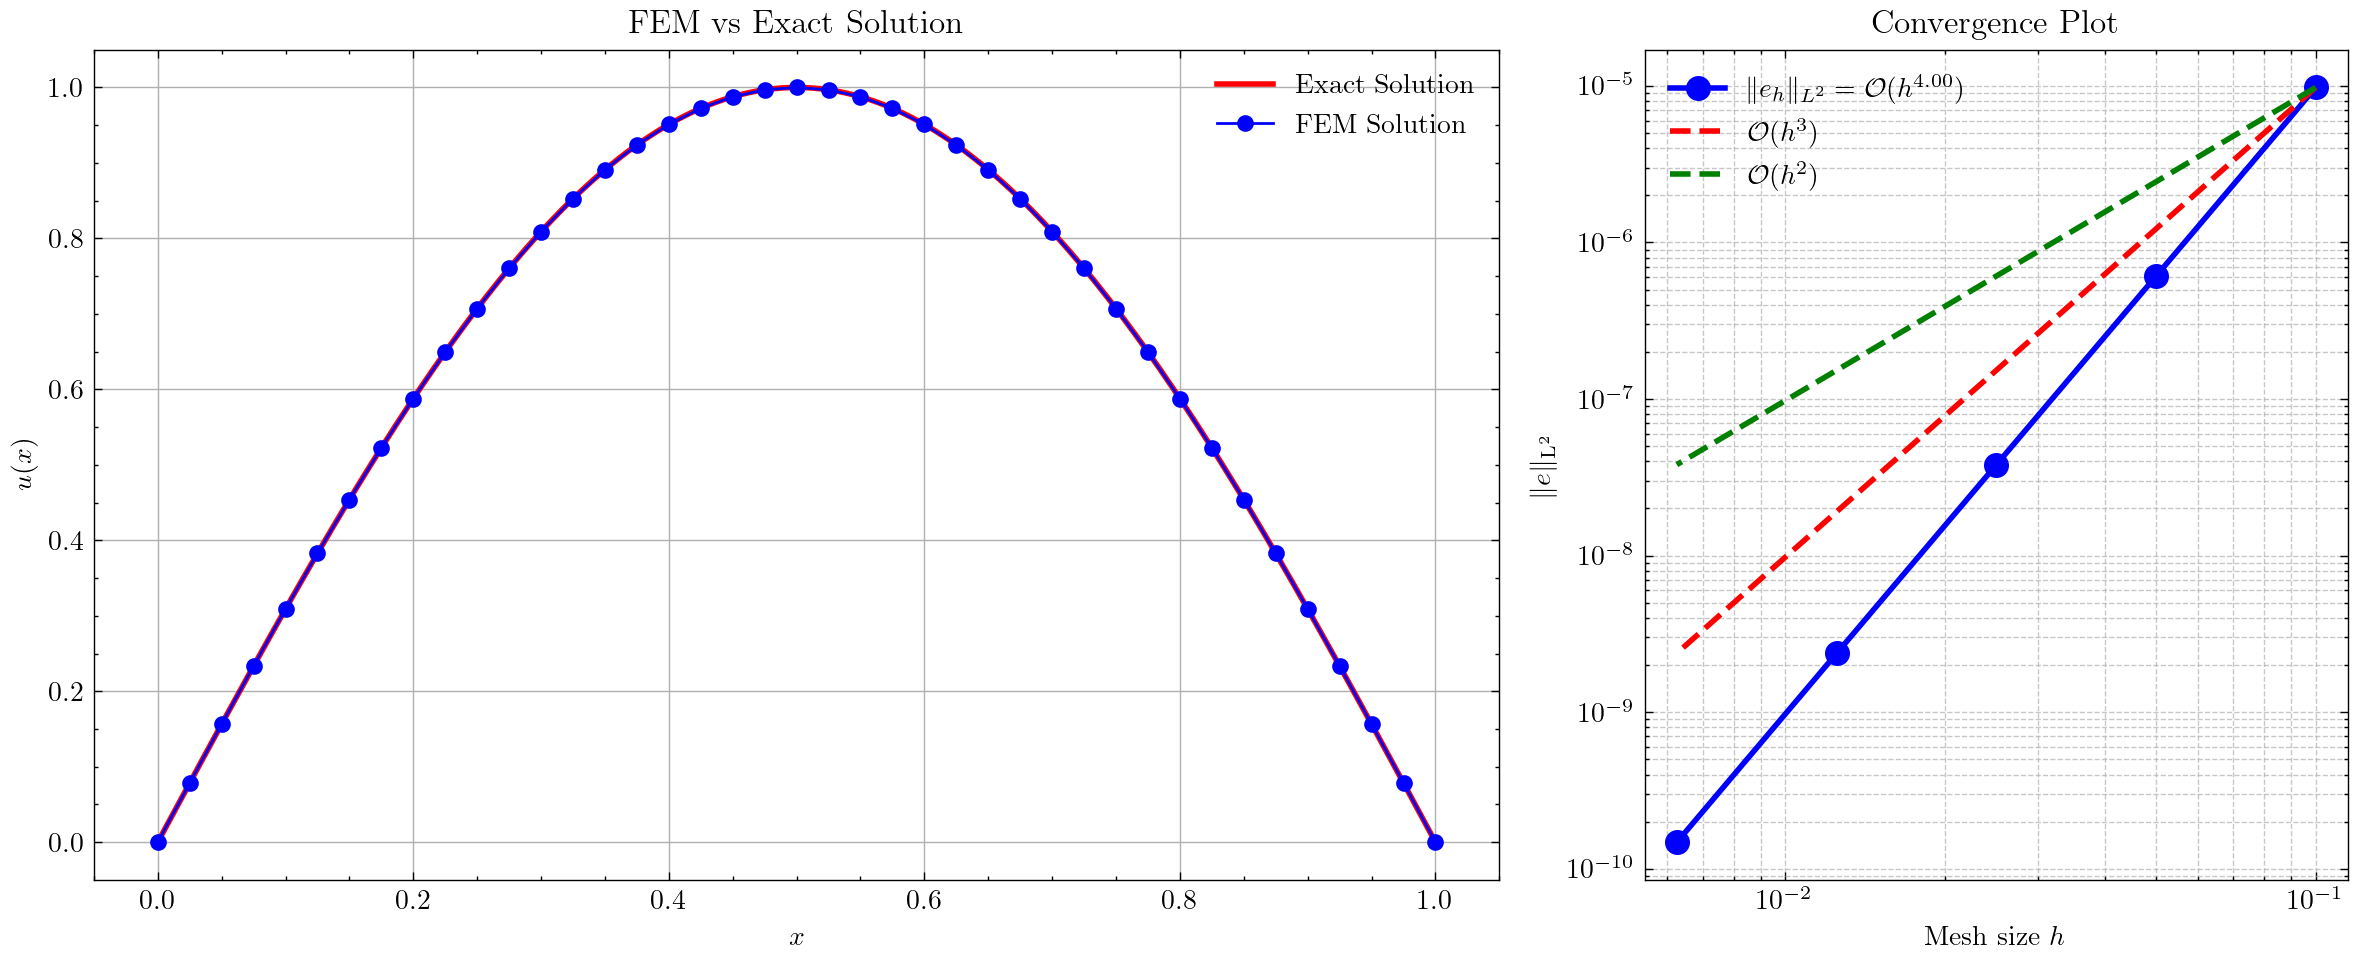
\includegraphics[width=0.9\textwidth]{figures/fem_plot_convergence_sine_M20.png}
	\caption{Finite element solution \(u_h(x)\) (blue dotted-solid line) versus the exact solution \(u(x)=\sin(\pi x)\) (red solid line) for the smooth sine example with \(M=20\) quadratic elements.}
	\label{fig:solution_sine}
\end{figure}

\begin{table}[ht]
	\centering
	\begin{tabular}{|c|c|c|c|c|c|c|c|}
		\hline
		\rowcolor{blue!25!white} 
		\multicolumn{1}{|c|}{$M$} & \multicolumn{1}{c|}{$h$} & \multicolumn{3}{c|}{$L^2$ Norm} & \multicolumn{3}{c|}{$H^1$ Norm} \\
		\hline
		\rowcolor{blue!25!white} 
		& & Error & Rate & Ratio & Error & Rate & Ratio \\
		\hline
		2 & 5.00e-01 & 6.71e-03 & -- & -- & 1.08e-02 & -- & -- \\
		\rowcolor{blue!5!white}
		4 & 2.50e-01 & 3.89e-04 & 4.11 & 17.25 & 6.53e-04 & 4.04 & 16.49 \\
		8 & 1.25e-01 & 2.39e-05 & 4.03 & 16.29 & 4.05e-05 & 4.01 & 16.11 \\
		\rowcolor{blue!5!white}
		16 & 6.25e-02 & 1.48e-06 & 4.01 & 16.07 & 2.53e-06 & 4.00 & 16.03 \\
		32 & 3.12e-02 & 9.27e-08 & 4.00 & 16.02 & 1.58e-07 & 4.00 & 16.01 \\
		\rowcolor{blue!5!white}
		64 & 1.56e-02 & 5.79e-09 & 4.00 & 16.00 & 9.87e-09 & 4.00 & 16.00 \\
		128 & 7.81e-03 & 3.62e-10 & 4.00 & 16.02 & 6.17e-10 & 4.00 & 16.00 \\
		\rowcolor{blue!5!white}
		256 & 3.91e-03 & 2.12e-11 & 4.09 & 17.06 & 3.87e-11 & 4.00 & 15.95 \\
		\hline
	\end{tabular}
	\caption{$L^2$ and $H^1$-norm errors for the sine example using quadratic elements. The consistent error reduction by a factor of approximately 16 when $h$ is halved confirms fourth-order convergence in both norms. Overall convergence rates: $L^2 \approx 4.02$, $H^1 \approx 4.01$. Final error at finest resolution: $L^2 = 2.12 \times 10^{-11}$, $H^1 = 3.87 \times 10^{-11}$.}
	\label{tab:convergence_1}
\end{table}

\subsubsection*{Simple Poisson Problem}
Consider the simple test problem $-u''(x)= 1$ for $x\in [0,1]$ with \(u(0)=u(1)=0\). The exact solution is \(u(x) = \frac{1}{2}x(1-x)\).
\begin{figure}[H]
	\centering
	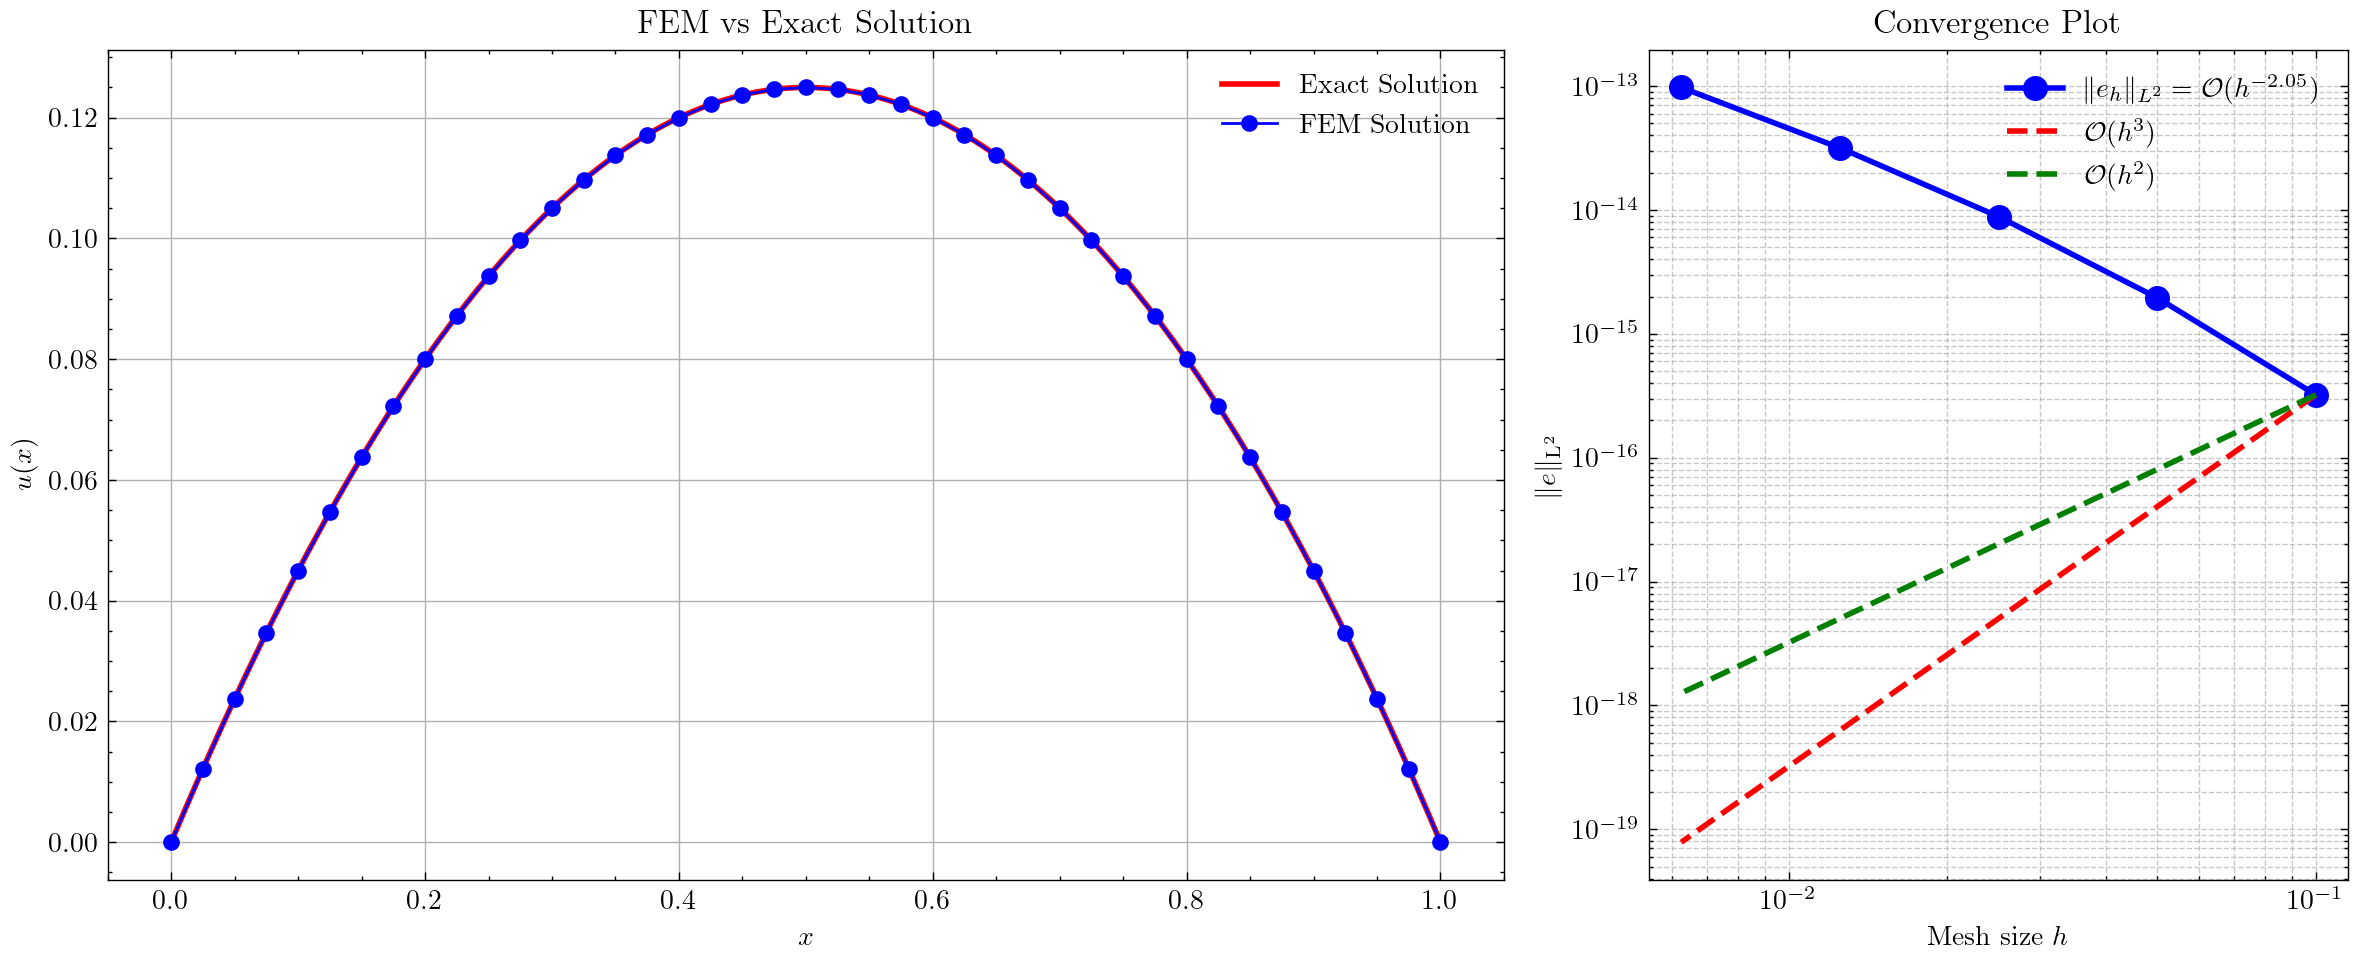
\includegraphics[width=0.85\textwidth]{figures/fem_plot_convergence_simple_M20.png}
	\caption{Finite element solution \(u_h(x)\) (blue dotted-solid line) versus the exact solution \(u(x)=\frac{1}{2}x(1-x)\) (red solid line) for the simple Poisson problem with \(M=20\) quadratic elements.}
	\label{fig:solution_simple}
\end{figure}
\begin{example}{Quadratic element mesh}{mesh_3}
	A mesh with $N=3$ elements has $(N+1)$ nodes and $N$ midpoints. Before boundary conditions, this yields $2N+1=7$ local shape functions. After enforcing $v(0)=v(1)=0$, we have $2N-1=5$ degrees of freedom.
	\begin{figure}[H]
		\centering
		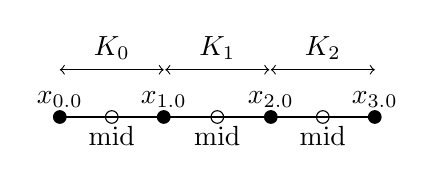
\begin{tikzpicture}[scale=4]
			% Draw interval [0,1]
			\draw[thick] (0,0) -- (1,0);

			% Nodes (filled circles)
			\foreach \x in {0,0.33,0.67,1}
			\draw[fill=black] (\x,0) circle (0.02)
			node[above] {$x_{\pgfmathparse{round(\x*3)}\pgfmathresult}$};

			% Midpoints (open circles) 
			\foreach \x in {0.165,0.5,0.835}
			\draw (\x,0) circle (0.02) node[below] {mid};

			% Element labels
			\foreach \x/\i in {0.165/0,0.5/1,0.835/2}
			\draw[<->] (\x-0.165,0.15) -- (\x+0.165,0.15)
			node[midway,above] {$K_{\i}$};
		\end{tikzpicture}
		\caption{Quadratic finite element mesh with $N=3$ elements showing nodes (solid dots) and element midpoints (open circles).}
	\end{figure}
\end{example}